% Standalone: method architecture M1--M7
\documentclass[tikz,border=6pt]{standalone}
\usepackage{amsmath}
\usetikzlibrary{arrows.meta,positioning,fit}
\begin{document}
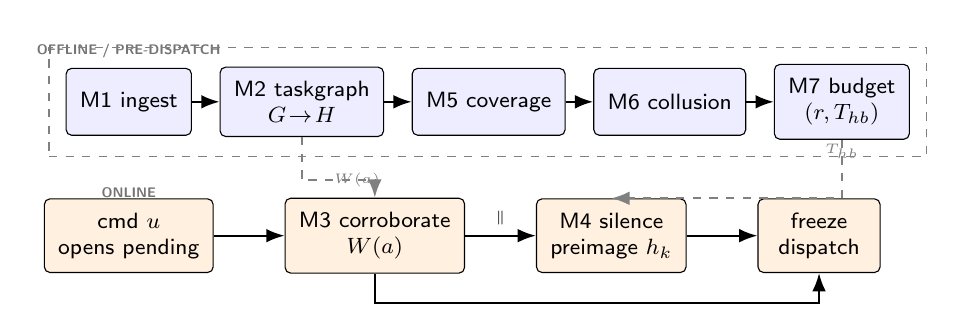
\begin{tikzpicture}[
  font=\sffamily\footnotesize,
  m/.style={draw, rounded corners=2pt, align=center, inner sep=5pt, minimum height=0.85cm, minimum width=1.55cm},
  off/.style={m, fill=blue!7},
  on/.style={m, fill=orange!12},
  arr/.style={-{Latex}, thick},
  lab/.style={font=\sffamily\tiny\bfseries, text=black!55},
]
\node[lab] at (0,2.35) {OFFLINE / PRE-DISPATCH};
\node[off] (m1) at (0,1.7) {M1 ingest};
\node[off, right=0.35cm of m1] (m2) {M2 taskgraph\\$G\!\to\!H$};
\node[off, right=0.35cm of m2] (m5) {M5 coverage};
\node[off, right=0.35cm of m5] (m6) {M6 collusion};
\node[off, right=0.35cm of m6] (m7) {M7 budget\\$(r,T_{hb})$};
\draw[arr] (m1) -- (m2);
\draw[arr] (m2) -- (m5);
\draw[arr] (m5) -- (m6);
\draw[arr] (m6) -- (m7);

\node[lab] at (0,0.55) {ONLINE};
\node[on] (cmd) at (0,0) {cmd $u$\\opens pending};
\node[on, right=0.9cm of cmd] (m3) {M3 corroborate\\$W(a)$};
\node[on, right=0.9cm of m3] (m4) {M4 silence\\preimage $h_k$};
\node[on, right=0.9cm of m4] (out) {freeze\\dispatch};
\draw[arr] (cmd) -- (m3);
\draw[arr] (m3) -- node[above, font=\tiny] {$\parallel$} (m4);
\draw[arr] (m3) -- ++(0,-0.85) -| (out);
\draw[arr] (m4) -- (out);

\draw[arr, dashed, gray] (m2.south) -- ++(0,-0.55) -| node[pos=0.15, right, font=\tiny, text=gray] {$W(a)$} (m3.north);
\draw[arr, dashed, gray] (m7.south) |- node[pos=0.25, above, font=\tiny, text=gray] {$T_{hb}$} (m4.north);

\node[draw, dashed, gray, fit=(m1)(m7), inner sep=6pt, label={[lab]above:}] {};
\end{tikzpicture}
\end{document}
